\documentclass[12pt]{article}
%\linespread{1}
\usepackage[margin=1.0in]{geometry}

\usepackage{amsmath}
\usepackage{amssymb}
\usepackage{multicol}
\usepackage{graphicx}
\usepackage{url}
\usepackage{fancyhdr}
\usepackage{color}

\newcommand\blfootnote[1]{%
  \begingroup
  \renewcommand\thefootnote{}\footnote{#1}%
  \addtocounter{footnote}{-1}%
  \endgroup
}

\title{Distributed Sampled Convex Problems}
\author{David Eckman (dje88) and Calvin Wylie (cjw278)}
\date{}

\begin{document}

%\noindent
\setlength{\parindent}{24pt}

\maketitle

\begin{abstract}
It is well-known that chance constrained programs are in general intractable because of the non-convexity of the feasible region and the requirement of prior information about the distribution of the uncertain parameters.
By solving a sampled convex program with sufficiently many samples of the uncertain parameters, one can find solutions that are feasible for the chance constrained program with high probability.
Sampled convex problems are more easily solved because they are characterized by a finite number of constraints and require only that one can obtain i.i.d. samples of the uncertain parameters.
However, the required number of samples may still result in a sampled convex program that is expensive to solve exactly.
We therefore consider a procedure for obtaining approximate solutions to these sampled convex programs by distributing the constraints across processors and solving smaller subproblems, followed by a consensus on the active constraints.
We experiment with a classical portfolio optimization problem and study the trade-offs that arise from this method: including wall-clock time, expected violation probability, and feasibility probability for the chance constrained program.
\end{abstract}

\blfootnote{Full source code and data for this paper is available at \url{https://github.com/calvinwylie/pscp}.}

\section*{Introduction}
Many real-world applications in areas as diverse as finance, energy, and emergency services can be modeled by chance constrained optimization problems \cite{bental09}.
For example, chance constraints can represent an acceptable level of risk in an investment or a fixed level of service that is guaranteed.
A typical chance-constrained program, \ref{ccp}, is given by
\begin{align}\label{ccp}
\begin{split}
\begin{aligned}
    & \underset{x \in \mathcal{X}}{\text{minimize}}
    & & c^T x \\
    & \text{subject to}
    & & \mathbb{P}\{f(x,\delta) \leq 0\} \geq 1-\epsilon.
\end{aligned}
\end{split} \tag{CCP$_\epsilon$}
\end{align}
where $\mathcal{X} \subseteq \mathbb{R}^n$ is compact, $\delta$ is an uncertain parameter distributed with probability measure $\mathbb{P}$ over an uncertainty set $\Delta \subseteq \mathbb{R}^d$, and $f:\mathcal{X} \times \Delta \mapsto \mathbb{R}$ is convex in $x$ for any fixed $\delta$.
The parameter $0 \leq \epsilon \leq 1$ represents the acceptable probability with which the constraint $f(x,\delta) \leq 0$ can be violated.
\ref{ccp} is notoriously intractable because the feasible region is non-convex for general probability measures.
Moreover, obtaining a convex approximation relies on knowing the distribution $\mathbb{P}$ (or at least the moments) a priori.

One method for finding solutions with ``good'' performance which are also feasible for \ref{ccp} with high probability is to take $N$ i.i.d. samples $(\delta_1, \ldots, \delta_N)$ and solve the corresponding sampled convex program, \ref{scp}:
\begin{align}\label{scp}
\begin{split}
\begin{aligned}
    & \underset{x \in \mathcal{X}}{\text{minimize}}
    & & c^T x \\
    & \text{subject to}
    & & f(x,\delta_i) \leq 0 \quad i = 1, \ldots, N.
\end{aligned}
\end{split} \tag{SCP$_N$}
\end{align}
Notice that in contrast to \ref{ccp}, \ref{scp} is more tractable since it has a finite number of constraints and a convex feasible region. Note that we also need not explicitly know $\mathbb{P}$, but instead only need to be able to obtain i.i.d. samples from it.

Let $x_N^*$ denote the (random) solution to \ref{scp} obtained by taking $N$ samples.
for a fixed $x_N^*$, let $V(x_N^*) := \mathbb{P}\{\delta \in \Delta: f(x_N^*, \delta) > 0\}$ be the corresponding violation probability.
If $V(x_N^*) \leq \epsilon$, then $x_N^*$ is feasible for \ref{ccp}.

Sampled convex programs do not provide a guarantee that $V(x_N^*) \leq \epsilon$ for a given sample size $N$.
Instead, Calafiore and Campi \cite{campi05} proved that one can bound the number of samples needed to ensure that $\mathbb{P}^N\{V(x_N^*) > \epsilon\} \leq \beta$,  where $\mathbb{P}^N$ is the product probability measure.
That is, the optimal solution to \ref{scp} is feasible for \ref{ccp} with probability greater than $1 - \beta$.
Their bound of $N \geq 1/(\epsilon\beta) - 1$ is simple to calculate, but is quite loose in terms of asymptotics.
The bound was further tightened in \cite{campi06} to choosing $N$ to satisfy
\[ \mathbb{P}^N\{V(x_N^*) > \epsilon\} \leq \binom{N}{d}(1-\epsilon)^{N-d}. \]
and then later by Campi and Garatti in \cite{campi08} to the solution of a binomial equation:
\[ \mathbb{P}^N\{V(x_N^*) > \epsilon\} = \sum_{i=0}^{d-1} \binom{N}{i} \epsilon^i (1-\epsilon)^{N-i}. \]
Note that all of these bounds are independent of the distribution $\mathbb{P}$, which means that $N$ can be calculated without prior knowledge of $\mathbb{P}$.
Even for modest $\epsilon$ and $\beta$, the required $N$ may be large enough that the resulting \ref{scp} instance is very computationally expensive to solve exactly, especially if the number of decision variables, $n$, is also large.

One idea for addressing this challenge is to decompose \ref{scp} into smaller sampled convex programs to be solved in parallel before forming some consensus across the subproblems.
Because the subproblems have only a fraction of the constraints, they can potentially be solved much quicker than the full \ref{scp} problem.
However, because each subproblem is only considering a subset of the constraints, there is a loss associated with this simplification: the solution returned will likely violate some of the constraints of \ref{scp} and therefore is less likely to be a feasible solution for \ref{ccp}.
But for some applications, the speedup in terms of time to solution due to parallelism may be worth the decrease in the probability that the solution is \ref{ccp}-feasible.
%In particular, we would like to study how much is lost with respect to \ref{ccp} feasibility by taking the active constraints from the subproblems and solving a final sampled convex program with these constraints.

\section*{Parallel Procedure for \ref{scp}}
To motivate our proposed procedure, recall that a constraint $\{ x: f(x) \leq 0 \}$ is \emph{active} at $\bar{x}$ if $f(\bar{x}) = 0$. Assuming some regularity conditions, a feasible convex program in $n$ dimensional space will have at most $n$ active constraints at the optimal solution.
Therefore the problem of finding an optimal solution to \ref{scp} can be viewed as the problem of identifying the $n$ active constraints at the optimal solution.

A recent paper by Carlone et al. \cite{carlone2014} studies solving large-scale convex programs in a distributed fashion.
It assumes a directed graph topology on the communication network connecting a set of processors.
Initially, each processor is given a subset of the constraints of the master problem with which it solves a convex subproblem.
It then identifies the active constraints at that solution and passes them to other processors according to the network topology.
Each processor receives the incoming constraints and resolves a convex subproblem with their original set of constraints plus the new constraints.
It was proven that after an almost surely finite number of iterations, all processors will reach a consensus about which constraints are active at the optimal solution to the master problem.
Note that the objective in \cite{carlone2014} is to recover the exact solution to the convex program, whereas we are interested in finding an approximate solution in far less time.

In practice, this procedure would take far too long to run to completion, especially since there is no bound on the number of iterations needed for consensus.
%The only instance you would fully run a procedure like this is if the master problem is too large to solve with existing software.
Instead, we will consider a variation of this procedure which only runs for two iterations and in which the topology of the communication network is a star graph in which all ``worker'' processors pass active constraints to a `master'' processor.
Because there are only two iterations, the solutions returned will likely not be the exact solution to \ref{scp}.
However this approximate solution can be calculated in less time, and thus it may be worth a loss in the probability of being a \ref{ccp}-feasible solution.

Suppose that we have available one master processor and $p$ worker processors.
For simplicity, suppose that $N = mp$ for some positive integer $m > n$.
Our proposed procedure is as follows:

\bigskip
\textbf{Parallel \ref{scp} Procedure}
\begin{enumerate}
\item Aquire $N$ i.i.d. samples $\delta_1, \ldots, \delta_N$.

\item For each worker processor $1 \leq j \leq p$, solve the subproblem
\begin{equation*}
\begin{aligned}
    & \underset{x \in \mathcal{X}}{\text{minimize}}
    & & c^T x \\
    & \text{subject to}
    & & f(x,\delta_i) \leq 0 \quad i = m(j-1) + 1, \ldots, mj.
\end{aligned}
\end{equation*}
Let $\tilde{x}_j$ denote the corresponding optimal solution.
Determine the set of active constraints at the optimal solution $\tilde{x}_j$.
Assuming that each sampled convex program is fully-supported with probability one (i.e. that there are $n$ active constraints),
label the samples corresponding to these constraints $\delta_{(1)}^j, \ldots, \delta_{(n)}^j$.
Pass the set of active constraints to the master processor.

\item On the master processor, solve the sampled convex program
\begin{equation*}
\begin{aligned}
    & \underset{x \in \mathcal{X}}{\text{minimize}}
    & & c^T x \\
    & \text{subject to}
    & & f(x,\delta_{(i)}^j) \leq 0 \quad i = 1,\ldots,n \text{ and } j = 1,\ldots,p.
\end{aligned}
\end{equation*}
Let $\tilde{x}$ denote the corresponding optimal solution.
\end{enumerate}

Changing the number of processors $p$ affects the sizes of boths the first-stage subproblems and the second stage master problem.
With more processors, the subproblems are smaller, but the total number of constraints passed to the master program ($np$) is larger.
This will impact the time to solution (wall-clock time) of the procedure in two conflicting ways.
And as the number of constraints in the master problem increases, we would expect $\mathbb{P}^N\{V(\tilde{x}) > \epsilon\}$ to decrease.
The main research question of this study will be: \textit{given these trade-offs, what is the optimal number of processors to use?}

We will also consider another version of this problem.
Assume that we are willing to commit to the wall-clock time needed to solve \ref{scp} exactly.
But instead of solving \ref{scp} we want to use the time to take more than $N$ samples and apply the distributed procedure in hopes of increasing the probability that the returned solution is feasible for \ref{ccp}.
\textit{What then are the best number of processors and number of constraints per processor?}

\section*{Example Problem}

We consider the classical portfolio optimization problem of selecting an allocation $y$ for investing one dollar over $n$ assets with uncertain returns $r_i$ for $i = 1, \ldots, n$.
Of these assets, we assume that the $n$th asset has a fixed payout; it might, for example, represent a bond with a certain return.
Each allocation of assets defines a portfolio.
Our objective is to choose a portfolio that maximizes the value-at-risk (VaR), denoted by $t$, for an acceptable risk level $\epsilon$.
Here VaR refers to the $\epsilon$-percentile of the distribution of returns for a particular portfolio as opposed to the (more traditional) $\epsilon$-percentile of the distribution of losses.

This setting gives rise to the following chance constrained program:
\begin{align}\label{Portfolioccp}
\begin{split}
\begin{aligned}
    & \underset{y, \,t}{\text{maximize}}
    & & t \\
    & \text{subject to}
    & & \mathbb{P}\left\{ \sum_{i=1}^{n-1} r_i y_i + r_n y_n \geq t \right\} \geq 1-\epsilon \\
    & & & \sum_{i=1}^n y_i = 1 \\
    & & & y_i \geq 0 \quad i = 1, \ldots, n.
\end{aligned}
\end{split} \tag{Portfolio CCP}
\end{align}

We will assume that the vector of uncertain returns $(r_1, \ldots, r_{n-1})$ is distributed according to a multivariate log-normal distribution with mean vector $\mu$ and covariance matrix $\Sigma$.
A log-normal distribution is a typical model for asset return because it is unimodal with support on the positive real line.
\textcolor{red}{In our experiment, we take $n=200$ and set the means and variances to be ...}
A more sophisticated approach might sample the returns from an empirical distribution function built from past data.


By taking samples $r^{(j)}$ for $j = 1, \ldots, N$, the corresponding sampled convex program is 
\begin{align}\label{Portfolioscp}
\begin{split}
\begin{aligned}
    & \underset{y, \,t}{\text{maximize}}
    & & t \\
    & \text{subject to}
    & & \sum_{i=1}^{n-1} r_i^{(j)} y_i + r_n^{(j)} y_n \geq t \quad j = 1, \ldots, N \\
    & & & \sum_{i=1}^n y_i = 1 \\
    & & & y_i \geq 0 \quad i = 1, \ldots, n.
\end{aligned}
\end{split} \tag{Portfolio SCP$_N$}
\end{align}


\ref{Portfolioscp} has several nice properties:
\begin{itemize}
\item The objective function and constraints of \ref{Portfolioscp} are linear. Therefore we can use standard linear programming techniques to solve the sampled convex program and subproblems.
\item Because of the fixed asset $n$, it is possible to easily find a basic feasible solution by taking $y_n = 1$, $y_i = 0$ for $i = 1, \ldots, n-1$ and $t = r_n$.
\item The feasible allocations $y$ sit within a unit simplex.
\end{itemize}

In our experiments, we took $\epsilon = 0.05$ and $\beta = 1 \times 10^{-5}$ and calculated a required sample size of $N = 5312$.

\section*{Implementation}

To solve our example portfolio optimization problem, we implemented a C interface to solve linear programs in parallel using the GNU Linear Programming Kit (GLPK) \footnote{\url{https://www.gnu.org/software/glpk/}}.
We chose to use the Simplex algorithm to solve our linear programs.  
As our contraints are very dense, interior point methods would likely be very slow.
To provide paralellism, we coded to the Message Passing Interface (MPI) standard.
The code was compiled with the Intel C compiler (icc), and experiments performed on a single 12-core Intel Xeon E5-2620 v3 processor.

Given a linear program with $m$ contraints and $n$ variables, the folklore on the simplex method is that it takes $O(m)$ pivots to reach the optimal solution for a ``typical'' linear program (the worst case is always $2^n - 1$).
Thus we should observe a roughly linear speedup when decomposing our sampled program into smaller subproblems.
Also given a problem where $m >> n$, it may make sense to solve the dual program instead (which can be done through the so-called Dual Simplex Algorithm), which has only $n$ constraints.

Figure \ref{fig:fig_simplex_time} shows some experimental timings for the simplex and dual simplex methods applied to our problem with $n = 200$ assets on a single core.
It shows the expected linear (in fact superlinear) increase in wall clock time with respect to the number of constraints.

However, we do not realize any speedup through solving the dual program.  
We guess this is because our sampled constraints are on average very similar to each other, and thus not as many pivots are needed to reach an optimal extreme point as would be required in a more ``standard'' linear program.

\begin{figure}[ht]
	\centering
		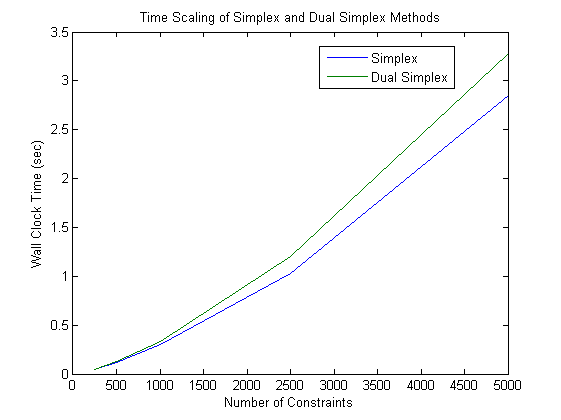
\includegraphics[scale=0.9]{../plot/figs/fig_simplex_time.png}
	\caption{Wall-Clock Times for Simplex and Dual Simplex Methods.}
	\label{fig:fig_simplex_time}
\end{figure}

\section*{Performance Analysis}

The program spends time in two main areas: communicating the constraint data through MPI, and solving the linear programs in GLPK.  
As these are two mature and heavily optimized libraries, manual performance tuning of the routines called would likely not lead to significant speedups.
We can however, reason about the overall performance of our program at a high level.

Assuming that the number of constraints is held constant, as Figure~\ref{fig:fig_simplex_time} suggests, we should see a linear decrease in the wall-clock time of the simplex algorithm when distributing the constraints across different processors.  
The time required for the final solve on the master processor (using active constraints) from the subproblems) should be small, as we can warm-start this optimization with an optimal basis from a subproblem.

However, as we increase the number of processors, the time to communicate the initial constraints (through an \texttt{MPI\_Scatter}) and the active constraints (through \texttt{MPI\_Gather}) will increase.
Through profiling, we verified that there is a roughly $O(p^2)$ relationship between communication time and the number of processors $p$.

This suggests that we should initially see decreases in wall-clock time as we add processors, but at some point the communication time will start to dominate the savings gained by splitting our problem.  
Figure~\ref{fig:wct_numproc} shows this experimentally.

\begin{figure}[ht]
    \centering
        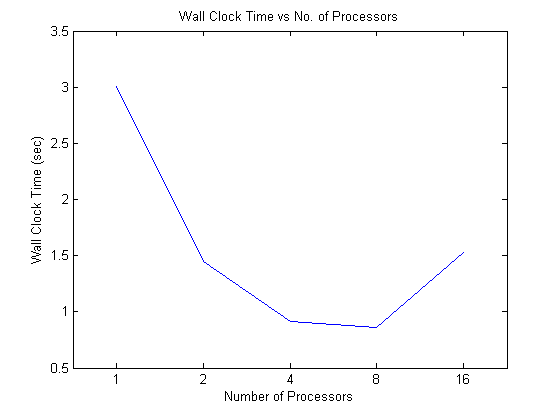
\includegraphics[scale=0.9]{../plot/figs/wct_numproc.png}
    \caption{Wall-Clock Times by Number of Processors.}
    \label{fig:wct_numproc}
\end{figure}


\section*{Experiments}
Let $\tilde{x} := (\tilde{y}, \tilde{t})$ denote the solution returned by running the parallel \ref{scp} procedure.
Even though the distribution $\mathbb{P}$ is known, calculating $V(\tilde{x})$ exactly is intractable.
Instead we estimated $V(\tilde{x})$ via Monte Carlo simulation, generating $R = 5000$ i.i.d. realizations of the returns $r$ and calculating
\[ \hat{V}(\tilde{x}) = \frac{1}{R} \sum_{j = 1}^R \mathbf{1}\left\{ \sum_{i=1}^{n-1} r_i^{(j)} \tilde{y}_i + r_n^{(j)} \tilde{y}_n < \tilde{t}\right\}. \]

We performed $M = 400$ macro-replications of this procedure, with corresponding solutions $\tilde{x}^{(k)}$ for $k = 1, \ldots, M$, and calculated the following point estimates of $\mathbb{E}[V(\tilde{x})]$ and $\mathbb{P}^N\{V(\tilde{x}) > \epsilon\}$:
\[ \widehat{\mathbb{E}[V(\tilde{x})]} := \frac{1}{M} \sum_{k=1}^M \hat{V}(\tilde{x}^{(k)}), \]
and
\[ \widehat{\mathbb{P}^N\{V(\tilde{x}) > \epsilon\}} := \frac{1}{M} \sum_{i=1}^M \mathbf{1}\left\{\hat{V}(\tilde{x}) > \epsilon\right\}. \]
We used the Clopper-Pearson exact binomial test to form approximate confidence intervals for these two performance measures.

When we divided the 5312 constraints evenly among $p$ processors, our estimates for $\mathbb{E}[V(\tilde{x})]$ and $\mathbb{P}^N\{V(\tilde{x}) > \epsilon\}$ are shown in Figures~\ref{fig:expviolprob_numproc} and \ref{fig:probviolprobgreateps_numproc}.

%\begin{figure}[ht]
	%\centering
		%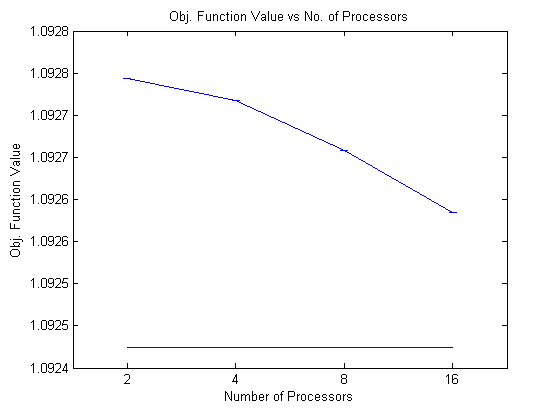
\includegraphics{../plot/figs/objfnval_num_proc.png}
	%\caption{VaR $\tilde{t}$ by Number of Processors}
	%\label{fig:objfnval_num_proc}
%\end{figure}
%
%\begin{figure}[ht]
	%\centering
		%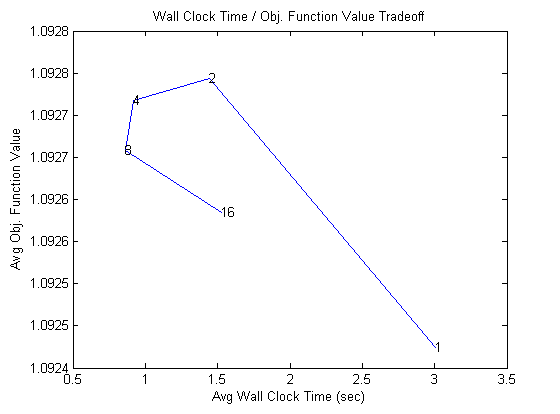
\includegraphics{../plot/figs/wct_objfnval_frontier.png}
	%\caption{Trade-off between Time and VaR $\tilde{t}$}
	%\label{fig:wct_objfnval_frontier}
%\end{figure}

\begin{figure}[ht]
	\centering
		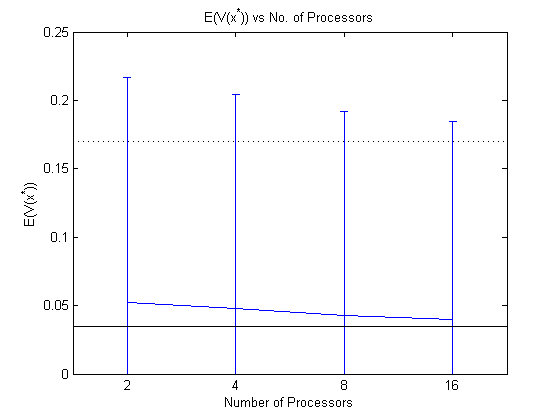
\includegraphics[scale=0.9]{../plot/figs/expviolprob_numproc.png}
	\caption{$\mathbb{E}[V(\tilde{x})]$ by Number of Processors.}
	\label{fig:expviolprob_numproc}
\end{figure}

\begin{figure}[ht]
	\centering
		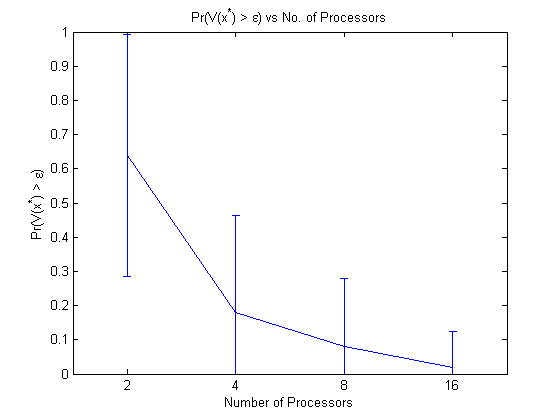
\includegraphics[scale=0.9]{../plot/figs/probviolprobgreateps_numproc.png}
	\caption{$\mathbb{P}^N\{V(\tilde{x}) > \epsilon \}$ by Number of Processors.}
	\label{fig:probviolprobgreateps_numproc}
\end{figure}

As can be seen in the Figures, even though at 4 processors and above, the violation probability $V(\tilde{x})$ is less than $\epsilon$ in expectation, the probability of \ref{ccp} contraint violation $\mathbb{P}^N\{V(\tilde{x}) > \epsilon \}$ is still very high (recall that we are aiming for $\mathbb{P}^N\{V(\tilde{x}) > \epsilon \} \leq \beta = 10^{-5}$).

Figure~\ref{fig:wct_probviolprobgreateps_frontier} shows the trade-off between wall-clock time and $\mathbb{P}^N\{V(\tilde{x}) > \epsilon \}$.  
This Figure shows that despite returning solutions with high probabilities of infeasibility, the parallel \ref{scp} procedure could run in a fraction of the time of the serial procedure.
This suggests that we could use some of the time savings to run the parallel procedure on more than $N$ samples, recovering solutions with feasibility probabilities competitive with the serial procedure, with still significant speedup.

\begin{figure}[ht]
	\centering
		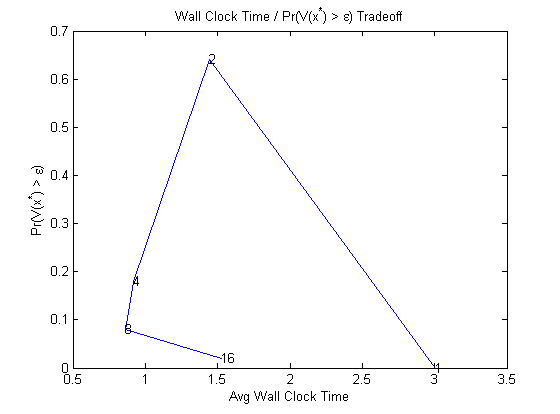
\includegraphics[scale=0.9]{../plot/figs/wct_probviolprobgreateps_frontier.png}
	\caption{Trade-off between Time and $\mathbb{P}^N\{V(\tilde{x}) > \epsilon \}$.}
	\label{fig:wct_probviolprobgreateps_frontier}
\end{figure}

In another set of experiments, we increased the number of samples given to each worker processor, typically doubling or quadrupaling.
For example, with $N = 5312$, running the parallel procedure with 8 processors means that each processor receives $N/8 = 664$ samples.
Here we ran the same procedure on 8 processors, except with 1328 and 2656 constraints for each processor (so now the total number of samples generated was 10624 and 21248).

Figure \ref{fig:wct_numconstraint} shows the wall-clock time results for the instances we tested.
Observe that the lowest point on each colored curve corresponds to the case of running the original problem of $N = 5312$ constraints.
From Figure \ref{fig:wct_numconstraint}, we can see the increases in wall-clock time for a fixed number of processors is again superlinear.
In addition, doubling the number of constraints per processor (for $p =4$, 8, and 16) appears to outperform the serial procedure in terms of wall-clock time and quadrupling the number of constraints per processor (for $p = 4$ and 8) has comparable times to the serial procedure.

\begin{figure}[ht]
	\centering
		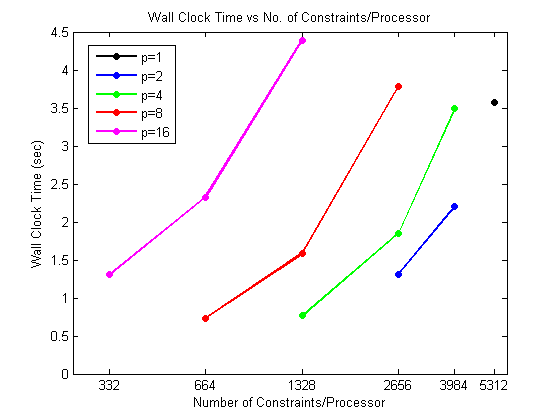
\includegraphics[scale=0.9]{../plot/figs/wct_numconstraint.png}
	\caption{Wall-Clock Times by Number of Constraints/Processor.}
	\label{fig:wct_numconstraint}
\end{figure}

Figures \ref{fig:expviolprob_numconstraint} and \ref{fig:probviolprobgreateps_numconstraint} show $\mathbb{E}[V(\tilde{x})]$ and $\mathbb{P}^N\{V(\tilde{x}) > \epsilon \}$, respectively, for these same instances.
On these plots, the highest point on each colored curve corresponds to the case of running the original problem.
As expected, both performance measures improve as the number of constraints per processor are increased.
It appears that doubling the number of constraints per processor is enough for the parallel procedure to match or surpass the performance of the serial procedure.

\begin{figure}[ht]
	\centering
		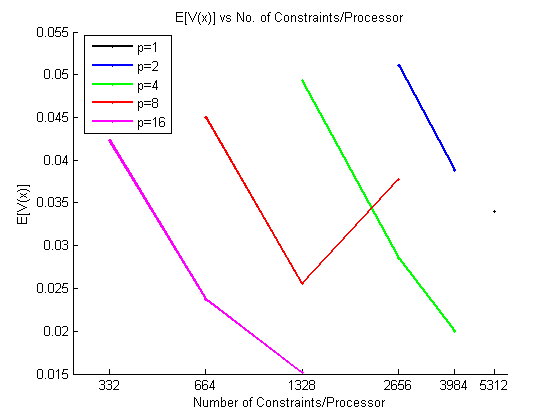
\includegraphics[scale=0.9]{../plot/figs/expviolprob_numconstraint.png}
	\caption{$\mathbb{E}[V(\tilde{x})]$ by Number of Constraints/Processor.}
	\label{fig:expviolprob_numconstraint}
\end{figure}

\begin{figure}[ht]
	\centering
		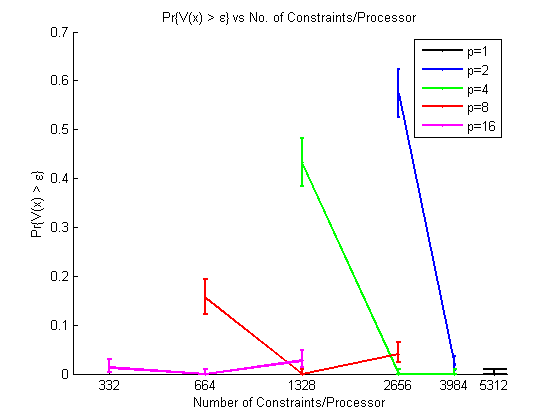
\includegraphics[scale=0.9]{../plot/figs/probviolprobgreateps_numconstraint.png}
	\caption{$\mathbb{P}^N\{V(\tilde{x}) > \epsilon \}$ by Number of Constraints/Processor.}
	\label{fig:probviolprobgreateps_numconstraint}
\end{figure}

Finally, the wall-clock time and $\mathbb{P}^N\{V(\tilde{x}) > \epsilon \}$ are shown together in Figure \ref{fig:wct_probviolprobgreateps_frontier_constraint}.
Each colored line represents a frontier for a fixed number of processors where the left-point on each curve is the original problem.
The number of constraints per processor increases as one moves to the right along each curve.
Based on this plot, an ``optimal'' number of configuration appears to be 8 processors with 1328 constraints per processor (the middle red point) because it attains the $\mathbb{P}^N\{V(\tilde{x}) > \epsilon \}$ of the serial solution in less than half the time.

\begin{figure}[ht]
	\centering
		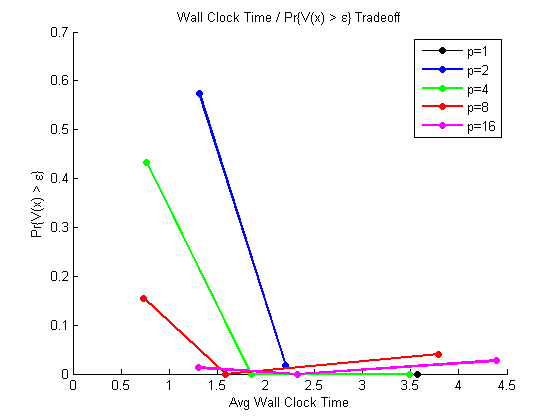
\includegraphics[scale=0.9]{../plot/figs/wct_probviolprobgreateps_frontier_constraint.png}
	\caption{Trade-off between Time and $\mathbb{P}^N\{V(\tilde{x}) > \epsilon \}$}
	\label{fig:wct_probviolprobgreateps_frontier_constraint}
\end{figure}

\section*{Conclusions}
For a modest-sized portfolio optimization problem, we observed that parallelism can dramatically reduce the run time with some loss in \ref{ccp} feasibility.
We believe that for more complex sampled convex programs---those with more decision variables and constraints or those of harder complexity than linear programs---the benefits of a distributed approach would be even more pronounced.
In our MPI implementation we observe marginally decreasing gains in run-time performance due to increased communication and the need to solve a larger second-stage problem.
When we experimented with adjusting the number of constraints per processor, our main conclusion was that one can typically sample twice as much while achieving faster run-times and \ref{ccp}-feasibility competitive with the serial procedure.


\section*{Open Extensions}
If we had more time, there are a number of open areas we would have wanted to explore:
\begin{itemize}
\item Experiment on an actual financial data set with forecasts for asset returns.
\item Compare the quality of the solution returned by our procedure with other solutions found by solving over convex inner approximations of the \ref{ccp} feasible region.
\item Extend our procedure to run multiple iterations of the worker/master sequence in hopes of better recovering the optimal active constraints.
\item Test for large problem sizes and other problems whose solution methods are of harder complexity than linear programming.
\end{itemize}

%We intend to conduct experiments on the performance of the parallel procedure versus the traditional serial \ref{scp} procedure.
%For measures of performance of the solutions $x^*$ and $x^{**}$, we will look at the objective function values, the expected violation probabilities, and the probabilities that the violations probabilities are greater than $\epsilon$.
%We will make comparisons based on both the total number of samples and the total wall-clock times of the two procedures.
%
%We will also experiment with variations of the basic procedure.
%One variation would involve communicating the support constraints of the master's problem back to the slaves and doing new sampling before solving new subproblems for each slaves.
%This could be done over a number of iterations and we could study the performance of the returned solutions at each iteration.
%
%Another variation would again involve communicating support constraints of the master's problem back to the slaves, but instead of doing new sampling, we re-solve the subproblems with the additional shared support constraints.
%After sending the support constraints of these new subproblems to the master, we could perform one final solve and get a solution that is no worse than the previous.
%This is because passing support constraints from the master to the slaves would allow for constraints that were not previously support constraints to become support constraints.

\bibliographystyle{siam}
\bibliography{references} 

\end{document}